

\documentclass{langscibook}
\usepackage{tikz}
\usetikzlibrary{matrix, patterns, backgrounds}
\begin{document}
	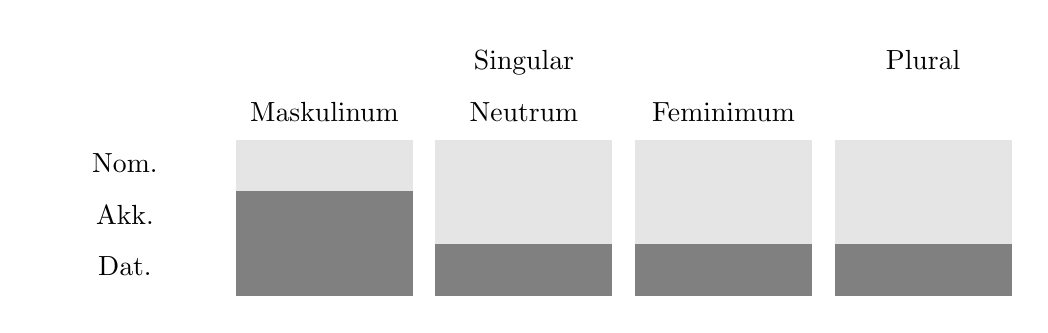
\begin{tikzpicture}
		\matrix [matrix of nodes,
		nodes in empty cells,
		column sep=3mm,
		align=center,
		nodes={text width=2cm, minimum height=1em, font=\strut}
		]
		(matrix)
		{ & & Singular & & Plural \\
				& Maskulinum & Neutrum & Feminimum & \\ 
			Nom.& & & & \\
			Akk.& & & & \\
			Dat.& & & & \\
		};
		\fill [fill=gray!20] 
		(matrix-3-2.north west) rectangle (matrix-3-2.south east);
		\fill [fill=gray]
		(matrix-4-2.north west) rectangle (matrix-5-2.south east);
		\fill [fill=gray!20] 
		(matrix-3-3.north west) rectangle (matrix-3-3.south east);
		\fill [fill=gray]
		(matrix-5-3.north west) rectangle (matrix-5-3.south east);
		\fill [fill=gray!20] 
		(matrix-4-3.north west) rectangle (matrix-4-3.south east);
		\fill [fill=gray]
		(matrix-5-4.north west) rectangle (matrix-5-4.south east);
		\fill [fill=gray]
		(matrix-5-5.north west) rectangle (matrix-5-5.south east);
		\fill [fill=gray!20]
		(matrix-3-5.north west) rectangle (matrix-4-5.south east);
		\fill [fill=gray!20]
		(matrix-3-4.north west) rectangle (matrix-4-4.south east);
	\end{tikzpicture}
\end{document}